\section{Deep Learning}

In the field of machine learning, the first models you
are often introduced to are those for regression
and classification that utilize linear
combinations of fixed basis functions.
According to \cite{Bishop:2008aa},
these models possess useful analytical and computational properties,
but their practical applicability is constrained 
since the their capacity is limited to linear functions
and they cannot understand the interaction between any two input variables.
This leads to problems such as the curse of dimensionality,
where the number of possible interactions between variables grows exponentially
with the number of input variables.
To address large-scale problems, it is essential to adapt the basis functions
to the data, as demonstrated by support vector machines (SVMs).
Alternatively, one can fix the number of basis functions in advance while
allowing them to be adaptive, utilizing parametric forms for the basis
functions with parameter values adjusted during training.

The most successful example of this approach in pattern recognition is the
\textbf{feed-forward neural network},
also known as the multilayer perceptron (MLP).
\begin{figure}[h]
    \centering
    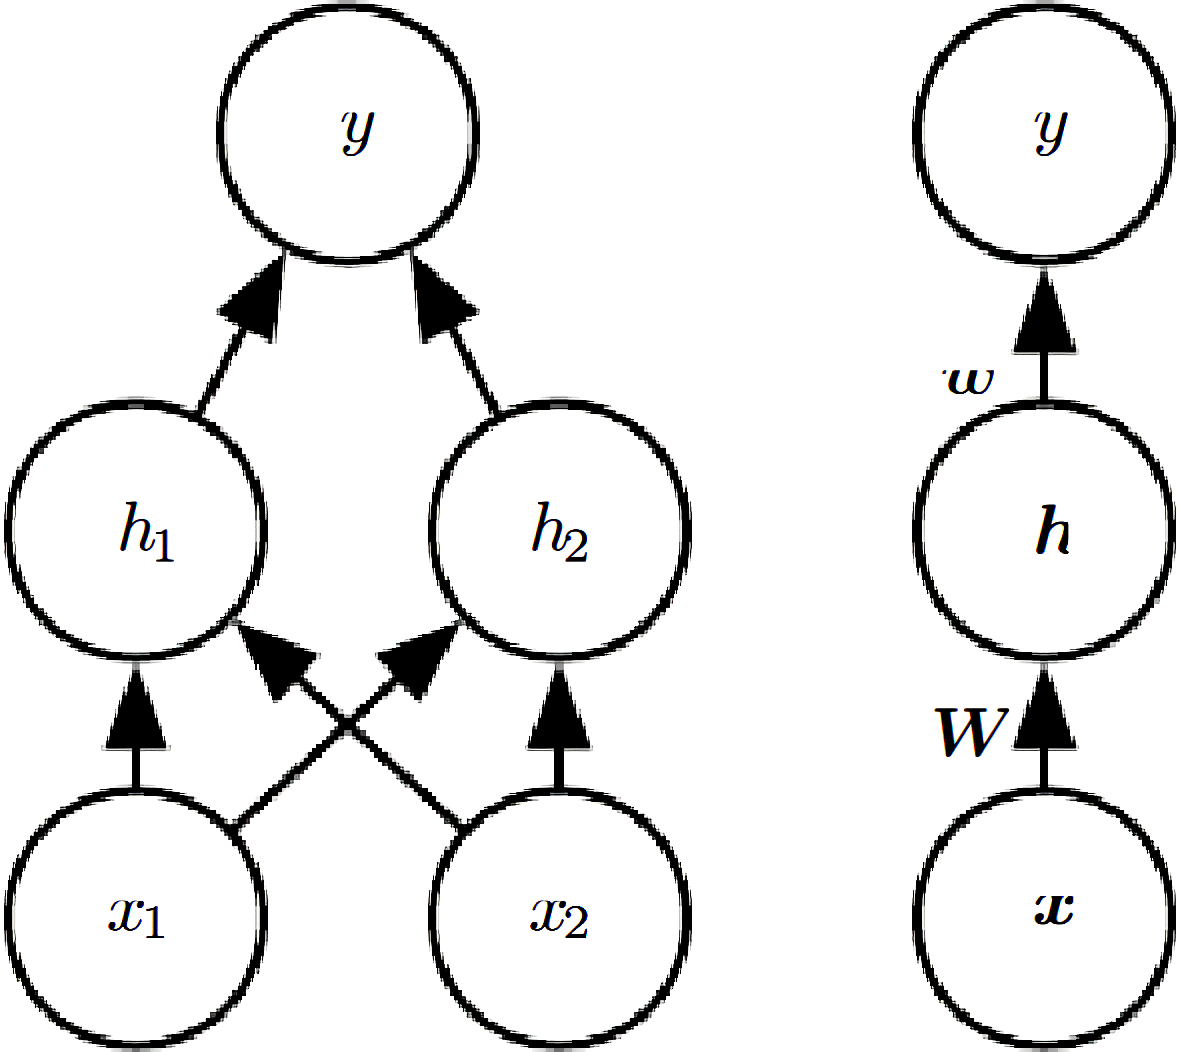
\includegraphics[width=.5\textwidth]{figures/ch3/1. mlp.png}
    \caption{A feed-forward neural network with one hidden layer, drawn 
    in two different styles.}
    \label{fig:mlp}
\end{figure}

The goal of a feedforward network is to approximate a specific function
\( f^* \) 
\cite{goodfellow2016deep}. For example, in a classification task,
\( y = f^*(x) \) maps an input \( x \) to a category \( y \).
A feedforward network defines a mapping \( y = f(x; \theta) \) and
learns the parameters \( \theta \) that yield the best approximation
of this function.

These models are called \textbf{feedforward} because information
flows unidirectionally from the input \( x \), through intermediate computations
defining \( f \), and ultimately to the output \( y \), without feedback loops.

They are called networks due to their structure, which involves composing
multiple functions together. Typically, this composition is represented
by a directed acyclic graph. For instance, functions
\( f^{(1)} \), \( f^{(2)} \), and \( f^{(3)} \) might be connected in
a chain to form \( f(x) = f^{(3)}(f^{(2)}(f^{(1)}(x))) \).

Functions \( f^{(1)} \), \( f^{(2)} \), and \( f^{(3)} \) must
be non linear, otherwise the composition would collapse into a single
linear function. These non-linear functions are
called \textbf{activation functions}.

During training, the network aims to make \( f(x) \) closely match \( f^*(x) \),
using noisy, approximate examples from the training data where each input
\( x \) is paired with a label \( y \approx f^*(x) \).
The training data directly specifies the output layer's behavior but
not the intermediate layers, which are called \textbf{hidden layers}
because their desired outputs are not provided by the training data.
The learning algorithm must determine how to best utilize these
hidden layers to approximate \( f^* \). Each hidden layer can be viewed
not just as a single vector-to-vector function, but as a set of parallel units,
each representing a vector-to-scalar function.

A feedforward network is called a \textbf{deep neural network} if it has
more than one hidden layer, the branch of machine learning that studies
deep neural networks is called \textbf{deep learning}.

To extend linear models to represent nonlinear functions of \( x \),
we can apply the linear model to a transformed
input \( \phi(x) \), where \( \phi \) is a nonlinear transformation.
The question then becomes how to choose the mapping \( \phi \).

The strategy of deep learning is to learn \( \phi \).
In this approach, we use a model
\[ y = f(x; \theta, w) = \phi(x; \theta)^\top w \]
Here, we have parameters \( \theta \) that are used to learn \( \phi \)
from a broad class of functions, and parameters \( w \) that map \( \phi(x) \)
to the desired output.
This approach allows for greater flexibility:
specifically, by using a broad family of functions
\( \phi(x; \theta) \), the human designer only needs to select the appropriate
general function family rather than finding precisely an exact function.

The \textbf{universal approximation theorem} \cite{HORNIK1989359}
tells us that regardless of what function
we are trying to learn, we know that a large MLP will be able to represent this
function. However, we are not guaranteed that the training algorithm will be able
to learn that function.

\section{Reinformcement Learning}


\section{Causal Inference}

\section{Generative Adversarial Networks}